\subsection{State-Machine}\label{sec:stateMachine}

Nachdem mit dem Einleitungskapitel ein kurzer Überblick geschaffen wurde, kann nun der Hauptteil der Software genauer betrachtet werden. Der gesamte Ablauf basiert auf einer klassischen State-Machine, die aufgrund von unterschiedlichen Parametern in die entsprechenden nächsten States springt. Das hat den Vorteil, dass sich das Programm stets in einem definierten Zustand befindet und mittels entsprechenden Parametern jeweils den nächsten Arbeitsschritt vordefiniert. Die Abbildung \ref{fig:completeStateMachine} zeigt das Gesamtkonzept der State-Machine. Anschliessend werden die einzelnen States genauer definiert und beschrieben.

\begin{figure}[htbp]
	\centering
	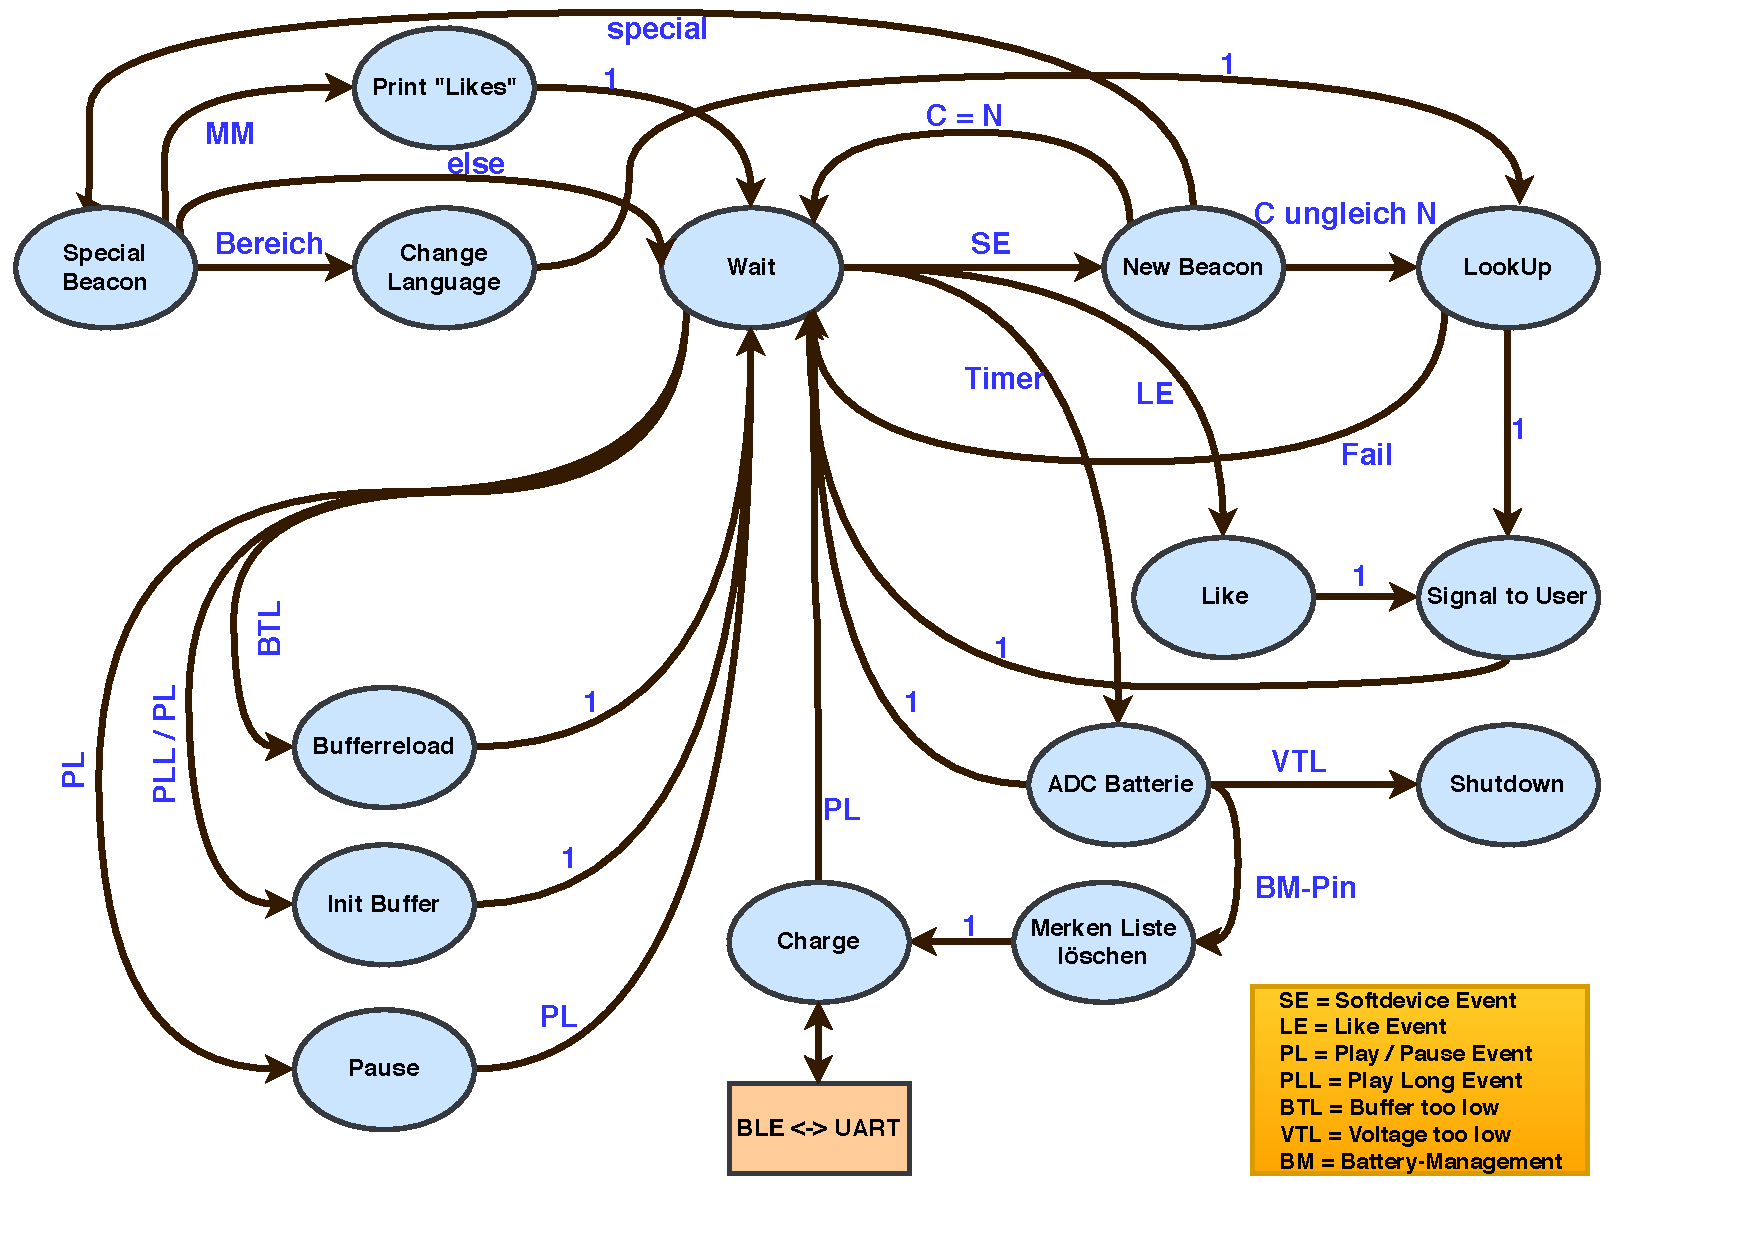
\includegraphics[width=1.15\textwidth]{Data/StateMachineFinal.pdf}
	\caption[Statemachine-Diagramm]{Statemachine im Überblick mit den einzelnen States und den Parametern}
	\label{fig:completeStateMachine}
\end{figure} 

\subsubsection*{State: Lookup}
In diesem State verschafft sich das Programm über die entsprechende Initialisierung Zugriff auf die SD-Karte der Anwendung. Falls der Mikrocontroller nicht auf die SD-Karte zugreifen kann, wird eine Fehlermeldung ausgegeben und die Funktion wird beendet. Anderenfalls wird dem Mikrocontroller signalisiert, dass der Zugriff geglückt ist und die eigentliche Funktion wird gestartet. Dazu werden die beiden Minor- und Majorzahlen in ein hexadezimales Zahlensystem gewandelt, welche dann als Vergleichskriterium verwendet werden. Falls die Nummer gefunden wird, kann das entsprechend zugehörige Audio-File über den Mikrocontroller ausgegeben werden. Verglichen wird jeweils zeilenweise, weshalb auch ein Fehlerhandling eingebaut wurde. Damit wird erkannt, ob sich das Textfile am Ende befindet. Somit lässt sich dann die Suche wiederholen, oder einen Fehler ausgeben. Die nachfolgende Abbildung \ref{fig:lookupState} zeigt den detaillierten Funktionsablauf im Lookup-State.

\begin{figure}[htbp!!!!]
	\centering
	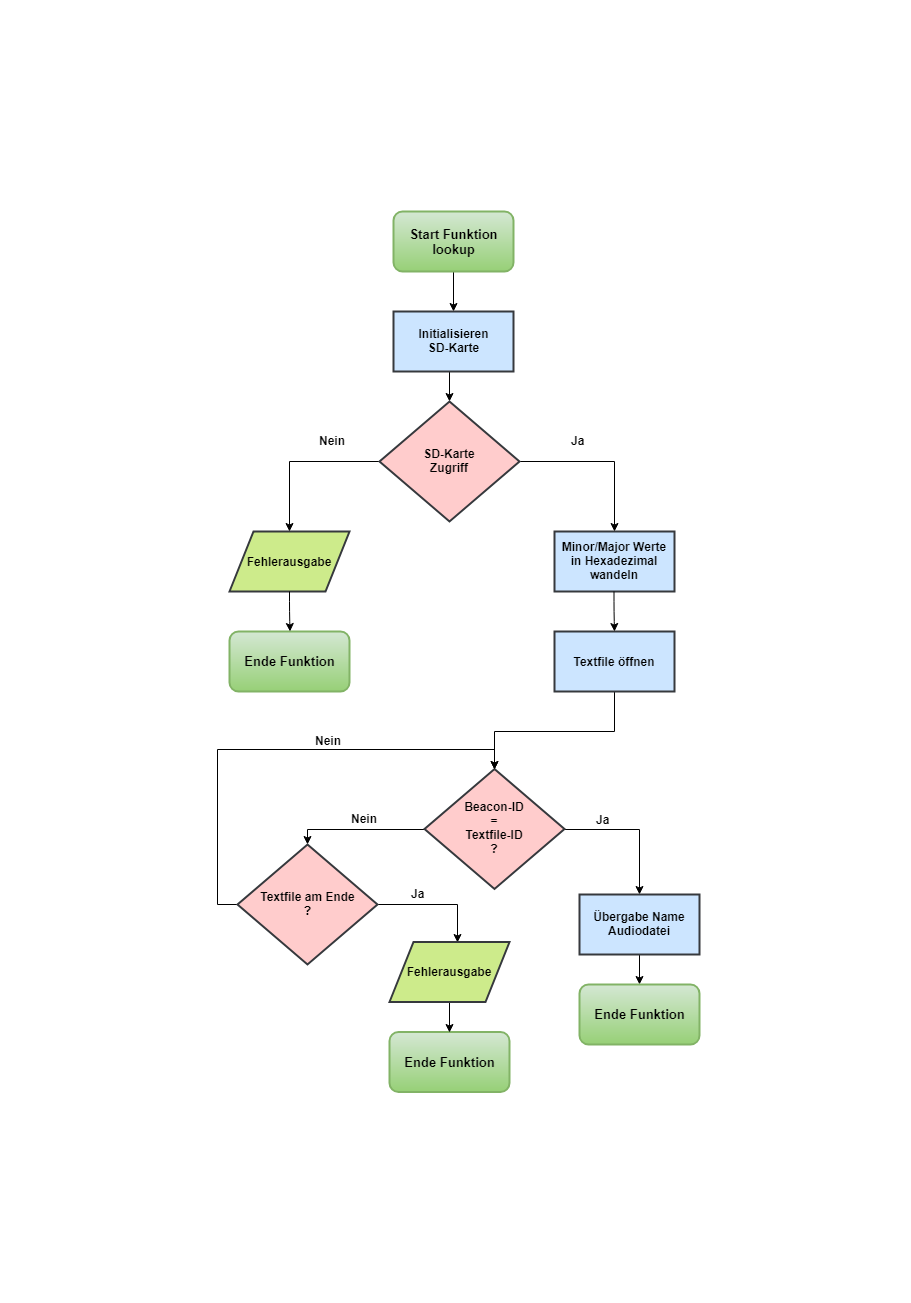
\includegraphics[width=0.5\textwidth]{Data/lookup_picture}
	\caption[Statemachine: lookup]{Lookup-State}
	\label{fig:lookupState}
\end{figure} 

\subsubsection*{State: Special Beacon}

\subsubsection*{State: Change Language}

\subsubsection*{State: Print \glqq Likes \grqq}

\subsubsection*{State: Wait}

\subsubsection*{State: New Beacon}

\subsubsection*{State: Like}

\subsubsection*{State: Signal to User}

\subsubsection*{State: ADC Battery}

\subsubsection*{State: Shutdown}

\subsubsection*{State: Merken Liste löschen}

\subsubsection*{State: Charge}

\subsubsection*{State: Pause}

\subsubsection*{State: Init Buffer}

\subsubsection*{State: Bufferreload}